
\documentclass[11pt]{article}
\usepackage[utf8]{inputenc}
\usepackage[left=0.2in, right=0.2in, top=0.4in, bottom=0.8in]{geometry}
\usepackage{graphicx}
\usepackage{booktabs}
\usepackage{xcolor}
\usepackage{colortbl}
\usepackage{tabularx}
\usepackage{tcolorbox}
\usepackage{titlesec}
\usepackage{microtype}
\usepackage{helvet}
\usepackage{hyperref}

\renewcommand{\familydefault}{\sfdefault}

\definecolor{primary}{RGB}{15, 23, 42}
\definecolor{accent}{RGB}{26, 54, 93}
\definecolor{cardbg}{RGB}{248, 250, 252}
\definecolor{cardborder}{RGB}{226, 232, 240}
\definecolor{posgreen}{RGB}{34, 197, 94}
\definecolor{negred}{RGB}{239, 68, 68}

\titleformat{\section}
  {\normalfont\Large\bfseries\color{primary}}
  {}{0em}
  {\color{accent}\vrule width 4pt\hspace{6pt}\color{primary}}

\begin{document}

%%%%%%%%%%%%%%%%%%%%%%%%%%%%%%%%%%%%%%%%%%%%
%% PAGE 1: 6-Month Strategy Deep Dive
%%%%%%%%%%%%%%%%%%%%%%%%%%%%%%%%%%%%%%%%%%%%

{\Huge \bfseries \color{accent} Athenee Lazarus Alpha AMC}\\[2.5em]

\begin{tcolorbox}[boxrule=0pt, leftrule=4pt, colframe=primary, colback=cardbg, sharp corners]
\textbf{\large Executive Summary} \\[4pt]
This product is a fund of hedge funds. The core idea is to pick strong performers that are uncorrelated, ensuring that returns keep up while overall volatility and max drawdown are significantly reduced. By blending distinct, non-overlapping strategies, the portfolio aims for robust risk-adjusted returns across market cycles.
\end{tcolorbox}

\subsection*{Monthly Returns Breakdown}
\begin{table}[h]
\centering
\renewcommand{\arraystretch}{1.3}
\begin{tabularx}{\textwidth}{l *{13}{>{\centering\arraybackslash}X}}
\toprule
\textbf{Year} & \textbf{Jan} & \textbf{Feb} & \textbf{Mar} & \textbf{Apr} & \textbf{May} & \textbf{Jun} & \textbf{Jul} & \textbf{Aug} & \textbf{Sep} & \textbf{Oct} & \textbf{Nov} & \textbf{Dec} & \textbf{YTD} \\
\midrule
2022 & \cellcolor{posgreen!2!white}0.2\% & \cellcolor{posgreen!22!white}2.3\% & \cellcolor{posgreen!21!white}2.1\% & \cellcolor{posgreen!19!white}2.0\% & \cellcolor{posgreen!26!white}2.7\% & \cellcolor{posgreen!31!white}3.2\% & \cellcolor{posgreen!34!white}3.5\% & \cellcolor{posgreen!27!white}2.7\% & \cellcolor{posgreen!19!white}2.0\% & \cellcolor{posgreen!26!white}2.7\% & \cellcolor{posgreen!20!white}2.0\% & \cellcolor{posgreen!31!white}3.1\% & \cellcolor{posgreen!100!white}32.5\% \\
2023 & \cellcolor{posgreen!13!white}1.3\% & \cellcolor{posgreen!11!white}1.1\% & \cellcolor{posgreen!21!white}2.2\% & \cellcolor{posgreen!19!white}1.9\% & \cellcolor{posgreen!32!white}3.2\% & \cellcolor{posgreen!23!white}2.4\% & \cellcolor{posgreen!24!white}2.5\% & \cellcolor{posgreen!12!white}1.2\% & \cellcolor{posgreen!13!white}1.3\% & \cellcolor{posgreen!11!white}1.2\% & \cellcolor{posgreen!23!white}2.4\% & \cellcolor{posgreen!16!white}1.6\% & \cellcolor{posgreen!100!white}24.8\% \\
2024 & \cellcolor{posgreen!18!white}1.8\% & \cellcolor{posgreen!10!white}1.0\% & \cellcolor{posgreen!30!white}3.0\% & \cellcolor{posgreen!13!white}1.4\% & \cellcolor{posgreen!17!white}1.7\% & \cellcolor{posgreen!13!white}1.3\% & \cellcolor{posgreen!18!white}1.9\% & \cellcolor{posgreen!19!white}1.9\% & \cellcolor{posgreen!9!white}1.0\% & \cellcolor{posgreen!17!white}1.7\% & \cellcolor{posgreen!21!white}2.2\% & \cellcolor{posgreen!16!white}1.6\% & \cellcolor{posgreen!100!white}22.7\% \\
2025 & \cellcolor{posgreen!19!white}1.9\% & \cellcolor{posgreen!14!white}1.4\% & \cellcolor{posgreen!20!white}2.0\% & \cellcolor{posgreen!20!white}2.1\% & \cellcolor{posgreen!11!white}1.2\% & \cellcolor{posgreen!6!white}0.7\% & \cellcolor{posgreen!22!white}2.2\% & \cellcolor{posgreen!17!white}1.7\% & \cellcolor{posgreen!23!white}2.4\% & \cellcolor{posgreen!30!white}3.1\% & \cellcolor{posgreen!22!white}2.2\% & \cellcolor{posgreen!17!white}1.8\% & \cellcolor{posgreen!100!white}25.1\% \\
2026 & \cellcolor{posgreen!12!white}1.2\% & \cellcolor{posgreen!11!white}1.1\% & \cellcolor{posgreen!21!white}2.2\% & \cellcolor{posgreen!11!white}1.1\% & - & - & - & - & - & - & - & - & \cellcolor{posgreen!57!white}5.8\% \\
\bottomrule
\end{tabularx}
\end{table}



\begin{minipage}[t]{0.48\textwidth}
\begin{tcolorbox}[colback=white, colframe=primary, title=\textbf{\large Performance \& Risk}, fonttitle=\sffamily\bfseries\large, arc=6pt, boxrule=1pt, toptitle=6pt, bottomtitle=6pt, left=0pt, right=0pt, top=0pt, bottom=0pt, colbacktitle=primary]
\renewcommand{\arraystretch}{1.8}
\begin{tabularx}{\textwidth}{>{\columncolor{white}}X >{\columncolor{white}}r}
\rowcolor{cardbg} \textbf{\textcolor{primary}{CAGR}} & \textcolor{primary}{25.59\%} \\
\textbf{\textcolor{primary}{Std}} & \textcolor{primary}{2.43\%} \\
\rowcolor{cardbg} \textbf{\textcolor{primary}{Proxy Sharpe}} & \textcolor{primary}{9.48} \\
\textbf{\textcolor{primary}{MDD}} & \textcolor{primary}{0.00\%} \\
\rowcolor{cardbg} \textbf{\textcolor{primary}{Calmar}} & \textcolor{primary}{-} \\
\textbf{\textcolor{primary}{Pos Months}} & \textcolor{primary}{100.0\%} \\
\end{tabularx}
\end{tcolorbox}
\end{minipage}\hfill
\begin{minipage}[t]{0.48\textwidth}
\begin{tcolorbox}[colback=white, colframe=primary, title=\textbf{\large Market Analysis}, fonttitle=\sffamily\bfseries\large, arc=6pt, boxrule=1pt, toptitle=6pt, bottomtitle=6pt, left=0pt, right=0pt, top=0pt, bottom=0pt, colbacktitle=primary]
\renewcommand{\arraystretch}{1.8}
\begin{tabularx}{\textwidth}{>{\columncolor{white}}X >{\columncolor{white}}r}
\rowcolor{cardbg} \textbf{\textcolor{primary}{Up Capture}} & \textcolor{primary}{0.51} \\
\textbf{\textcolor{primary}{Down Capture}} & \textcolor{primary}{-0.45} \\
\rowcolor{cardbg} \textbf{\textcolor{primary}{Alpha (t-stat)}} & \textcolor{primary}{23.00\% (19.05)} \\
\textbf{\textcolor{primary}{Beta}} & \textcolor{primary}{0.00} \\
\rowcolor{cardbg} \textbf{\textcolor{primary}{Corr SP500}} & \textcolor{primary}{0.02} \\
\textbf{\textcolor{primary}{N months}} & \textcolor{primary}{52} \\
\end{tabularx}
\end{tcolorbox}
\end{minipage}


\begin{figure}[h]
    \centering
    
\includegraphics[width=0.95\textwidth, height=0.35\textheight, keepaspectratio]{combined_growth_worst20_sp500.pdf}
\end{figure}



\clearpage
%%%%%%%%%%%%%%%%%%%%%%%%%%%%%%%%%%%%%%%%%%%%
%% PAGE 2: Fund Allocation & Strategy Descriptions
%%%%%%%%%%%%%%%%%%%%%%%%%%%%%%%%%%%%%%%%%%%%

\section*{Fund Allocation \& Strategy Descriptions}


\begin{tcolorbox}[colback=cardbg, colframe=cardborder, boxrule=0.5pt, arc=4pt, left=6pt, right=6pt, top=6pt, bottom=6pt]
    \begin{minipage}[c]{0.82\linewidth}
        \textbf{\textcolor{primary}{Crypto carry trade}} \\[4pt]
        \textcolor{primary}{Crypto carry trade market neutral fund.}
    \end{minipage}%
    \hfill
    \begin{minipage}[c]{0.15\linewidth}
        \centering
        \textbf{\Large \textcolor{accent}{6.7\%}}
    \end{minipage}
\end{tcolorbox}

\begin{tcolorbox}[colback=cardbg, colframe=cardborder, boxrule=0.5pt, arc=4pt, left=6pt, right=6pt, top=6pt, bottom=6pt]
    \begin{minipage}[c]{0.82\linewidth}
        \textbf{\textcolor{primary}{Quant FX / Metals trading}} \\[4pt]
        \textcolor{primary}{Trading-oriented fund on FX and precious metals with more than 4 trades per day.}
    \end{minipage}%
    \hfill
    \begin{minipage}[c]{0.15\linewidth}
        \centering
        \textbf{\Large \textcolor{accent}{6.7\%}}
    \end{minipage}
\end{tcolorbox}

\begin{tcolorbox}[colback=cardbg, colframe=cardborder, boxrule=0.5pt, arc=4pt, left=6pt, right=6pt, top=6pt, bottom=6pt]
    \begin{minipage}[c]{0.82\linewidth}
        \textbf{\textcolor{primary}{Chinese quant market neutral}} \\[4pt]
        \textcolor{primary}{Chinese equity market neutral fund that is strictly quant-driven.}
    \end{minipage}%
    \hfill
    \begin{minipage}[c]{0.15\linewidth}
        \centering
        \textbf{\Large \textcolor{accent}{6.7\%}}
    \end{minipage}
\end{tcolorbox}

\begin{tcolorbox}[colback=cardbg, colframe=cardborder, boxrule=0.5pt, arc=4pt, left=6pt, right=6pt, top=6pt, bottom=6pt]
    \begin{minipage}[c]{0.82\linewidth}
        \textbf{\textcolor{primary}{Distressed Debt}} \\[4pt]
        \textcolor{primary}{Fund investing in highly distressed debt and bond contracts.}
    \end{minipage}%
    \hfill
    \begin{minipage}[c]{0.15\linewidth}
        \centering
        \textbf{\Large \textcolor{accent}{6.7\%}}
    \end{minipage}
\end{tcolorbox}

\begin{tcolorbox}[colback=cardbg, colframe=cardborder, boxrule=0.5pt, arc=4pt, left=6pt, right=6pt, top=6pt, bottom=6pt]
    \begin{minipage}[c]{0.82\linewidth}
        \textbf{\textcolor{primary}{Quant high frequency}} \\[4pt]
        \textcolor{primary}{Market maker in Singapore investing in high-frequency strategies. They launched their open commingled fund for strategies that are highly scalable.}
    \end{minipage}%
    \hfill
    \begin{minipage}[c]{0.15\linewidth}
        \centering
        \textbf{\Large \textcolor{accent}{13.3\%}}
    \end{minipage}
\end{tcolorbox}

\begin{tcolorbox}[colback=cardbg, colframe=cardborder, boxrule=0.5pt, arc=4pt, left=6pt, right=6pt, top=6pt, bottom=6pt]
    \begin{minipage}[c]{0.82\linewidth}
        \textbf{\textcolor{primary}{Systematic multi asset}} \\[4pt]
        \textcolor{primary}{Smithson fund description.}
    \end{minipage}%
    \hfill
    \begin{minipage}[c]{0.15\linewidth}
        \centering
        \textbf{\Large \textcolor{accent}{13.3\%}}
    \end{minipage}
\end{tcolorbox}

\begin{tcolorbox}[colback=cardbg, colframe=cardborder, boxrule=0.5pt, arc=4pt, left=6pt, right=6pt, top=6pt, bottom=6pt]
    \begin{minipage}[c]{0.82\linewidth}
        \textbf{\textcolor{primary}{Quant Indian medium frequency}} \\[4pt]
        \textcolor{primary}{Indian-based fund investing in medium-frequency strategies across a lot of asset classes (intra-day trading with holdings of 2-3 hours). Founded by a team with strong prop trading desk experience who spun out to create this fund.}
    \end{minipage}%
    \hfill
    \begin{minipage}[c]{0.15\linewidth}
        \centering
        \textbf{\Large \textcolor{accent}{13.3\%}}
    \end{minipage}
\end{tcolorbox}

\begin{tcolorbox}[colback=cardbg, colframe=cardborder, boxrule=0.5pt, arc=4pt, left=6pt, right=6pt, top=6pt, bottom=6pt]
    \begin{minipage}[c]{0.82\linewidth}
        \textbf{\textcolor{primary}{Biotech focused}} \\[4pt]
        \textcolor{primary}{Adar1 fund description.}
    \end{minipage}%
    \hfill
    \begin{minipage}[c]{0.15\linewidth}
        \centering
        \textbf{\Large \textcolor{accent}{6.7\%}}
    \end{minipage}
\end{tcolorbox}

\begin{tcolorbox}[colback=cardbg, colframe=cardborder, boxrule=0.5pt, arc=4pt, left=6pt, right=6pt, top=6pt, bottom=6pt]
    \begin{minipage}[c]{0.82\linewidth}
        \textbf{\textcolor{primary}{FX Swap Arbitrage}} \\[4pt]
        \textcolor{primary}{FX Swap arbitrage}
    \end{minipage}%
    \hfill
    \begin{minipage}[c]{0.15\linewidth}
        \centering
        \textbf{\Large \textcolor{accent}{13.3\%}}
    \end{minipage}
\end{tcolorbox}

\begin{tcolorbox}[colback=cardbg, colframe=cardborder, boxrule=0.5pt, arc=4pt, left=6pt, right=6pt, top=6pt, bottom=6pt]
    \begin{minipage}[c]{0.82\linewidth}
        \textbf{\textcolor{primary}{Systematic Global Macro}} \\[4pt]
        \textcolor{primary}{Quant Global Macro with extremely well done risk management.}
    \end{minipage}%
    \hfill
    \begin{minipage}[c]{0.15\linewidth}
        \centering
        \textbf{\Large \textcolor{accent}{13.3\%}}
    \end{minipage}
\end{tcolorbox}

\clearpage

\section*{Detailed Fund Statistics}
\begin{table}[h]
\centering
\renewcommand{\arraystretch}{1.5}
\footnotesize
\begin{tabularx}{\textwidth}{l *{3}{>{\centering\arraybackslash}X} c *{8}{>{\centering\arraybackslash}X}}
\toprule
 & \textbf{CAGR} & \textbf{Std} & \textbf{Proxy Sharpe} & \textbf{MDD} & \textbf{Calmar} & \textbf{Pos Months} & \textbf{Up Capture} & \textbf{Down Capture} & \textbf{Alpha (t-stat)} & \textbf{Beta} & \textbf{Corr SP500} & \textbf{N months}\\
\midrule
\textbf{Crypto Carry} & 18.37\% & 5.43\% & 3.16 & -0.77\% & 23.91 & 92.5\% & 0.43 & -0.41 & 15.81\% (4.79) & 0.06 & 0.15 & 40 \\
\textbf{Quant FX} & 34.62\% & 18.63\% & 1.70 & -26.03\% & 1.33 & 69.6\% & 0.68 & -0.75 & 34.33\% (5.44) & -0.17 & -0.14 & 112 \\
\textbf{Chinese MN} & 20.55\% & 13.63\% & 1.45 & -10.84\% & 1.90 & 65.2\% & 0.39 & -0.60 & 20.53\% (4.86) & -0.06 & -0.06 & 135 \\
\textbf{Distr Debt} & 25.85\% & 11.81\% & 2.02 & -8.74\% & 2.96 & 78.1\% & 0.68 & -0.03 & 20.12\% (4.08) & 0.19 & 0.26 & 73 \\
\textbf{Quant HFT} & 21.33\% & 6.81\% & 2.89 & -1.39\% & 15.35 & 85.7\% & 0.45 & -0.68 & 20.33\% (4.01) & -0.03 & -0.05 & 28 \\
\textbf{Syst Multi Asset} & 47.09\% & 6.60\% & 5.97 & -0.63\% & 74.74 & 97.0\% & 0.79 & -1.06 & 39.92\% (13.68) & -0.03 & -0.08 & 67 \\
\textbf{Quant Indian} & 24.90\% & 7.36\% & 3.09 & -2.20\% & 11.33 & 84.4\% & 0.44 & -0.62 & 24.14\% (7.39) & -0.10 & -0.20 & 64 \\
\textbf{Biotech} & 34.92\% & 15.60\% & 2.02 & -10.63\% & 3.28 & 74.4\% & 0.88 & -0.18 & 26.38\% (4.60) & 0.31 & 0.34 & 86 \\
\textbf{FX Swap Arbitrage} & 29.08\% & 2.06\% & 12.53 & 0.00\% & - & 100.0\% & 0.64 & -0.85 & 26.17\% (17.36) & -0.02 & -0.12 & 27 \\
\textbf{Quant Global Macro} & 46.93\% & 14.41\% & 2.78 & -15.19\% & 3.09 & 86.9\% & 1.15 & -0.58 & 36.08\% (10.14) & 0.28 & 0.28 & 198 \\
\bottomrule
\end{tabularx}
\end{table}
\vspace{1em}
\begin{center}
    
\includegraphics[width=0.95\textwidth, height=0.4\textheight, keepaspectratio]{correlation.pdf}
\end{center}
\clearpage

\section*{Performance \& Returns}
The following visuals illustrate the fund-level statistics and the diversification benefits.

\begin{center}
    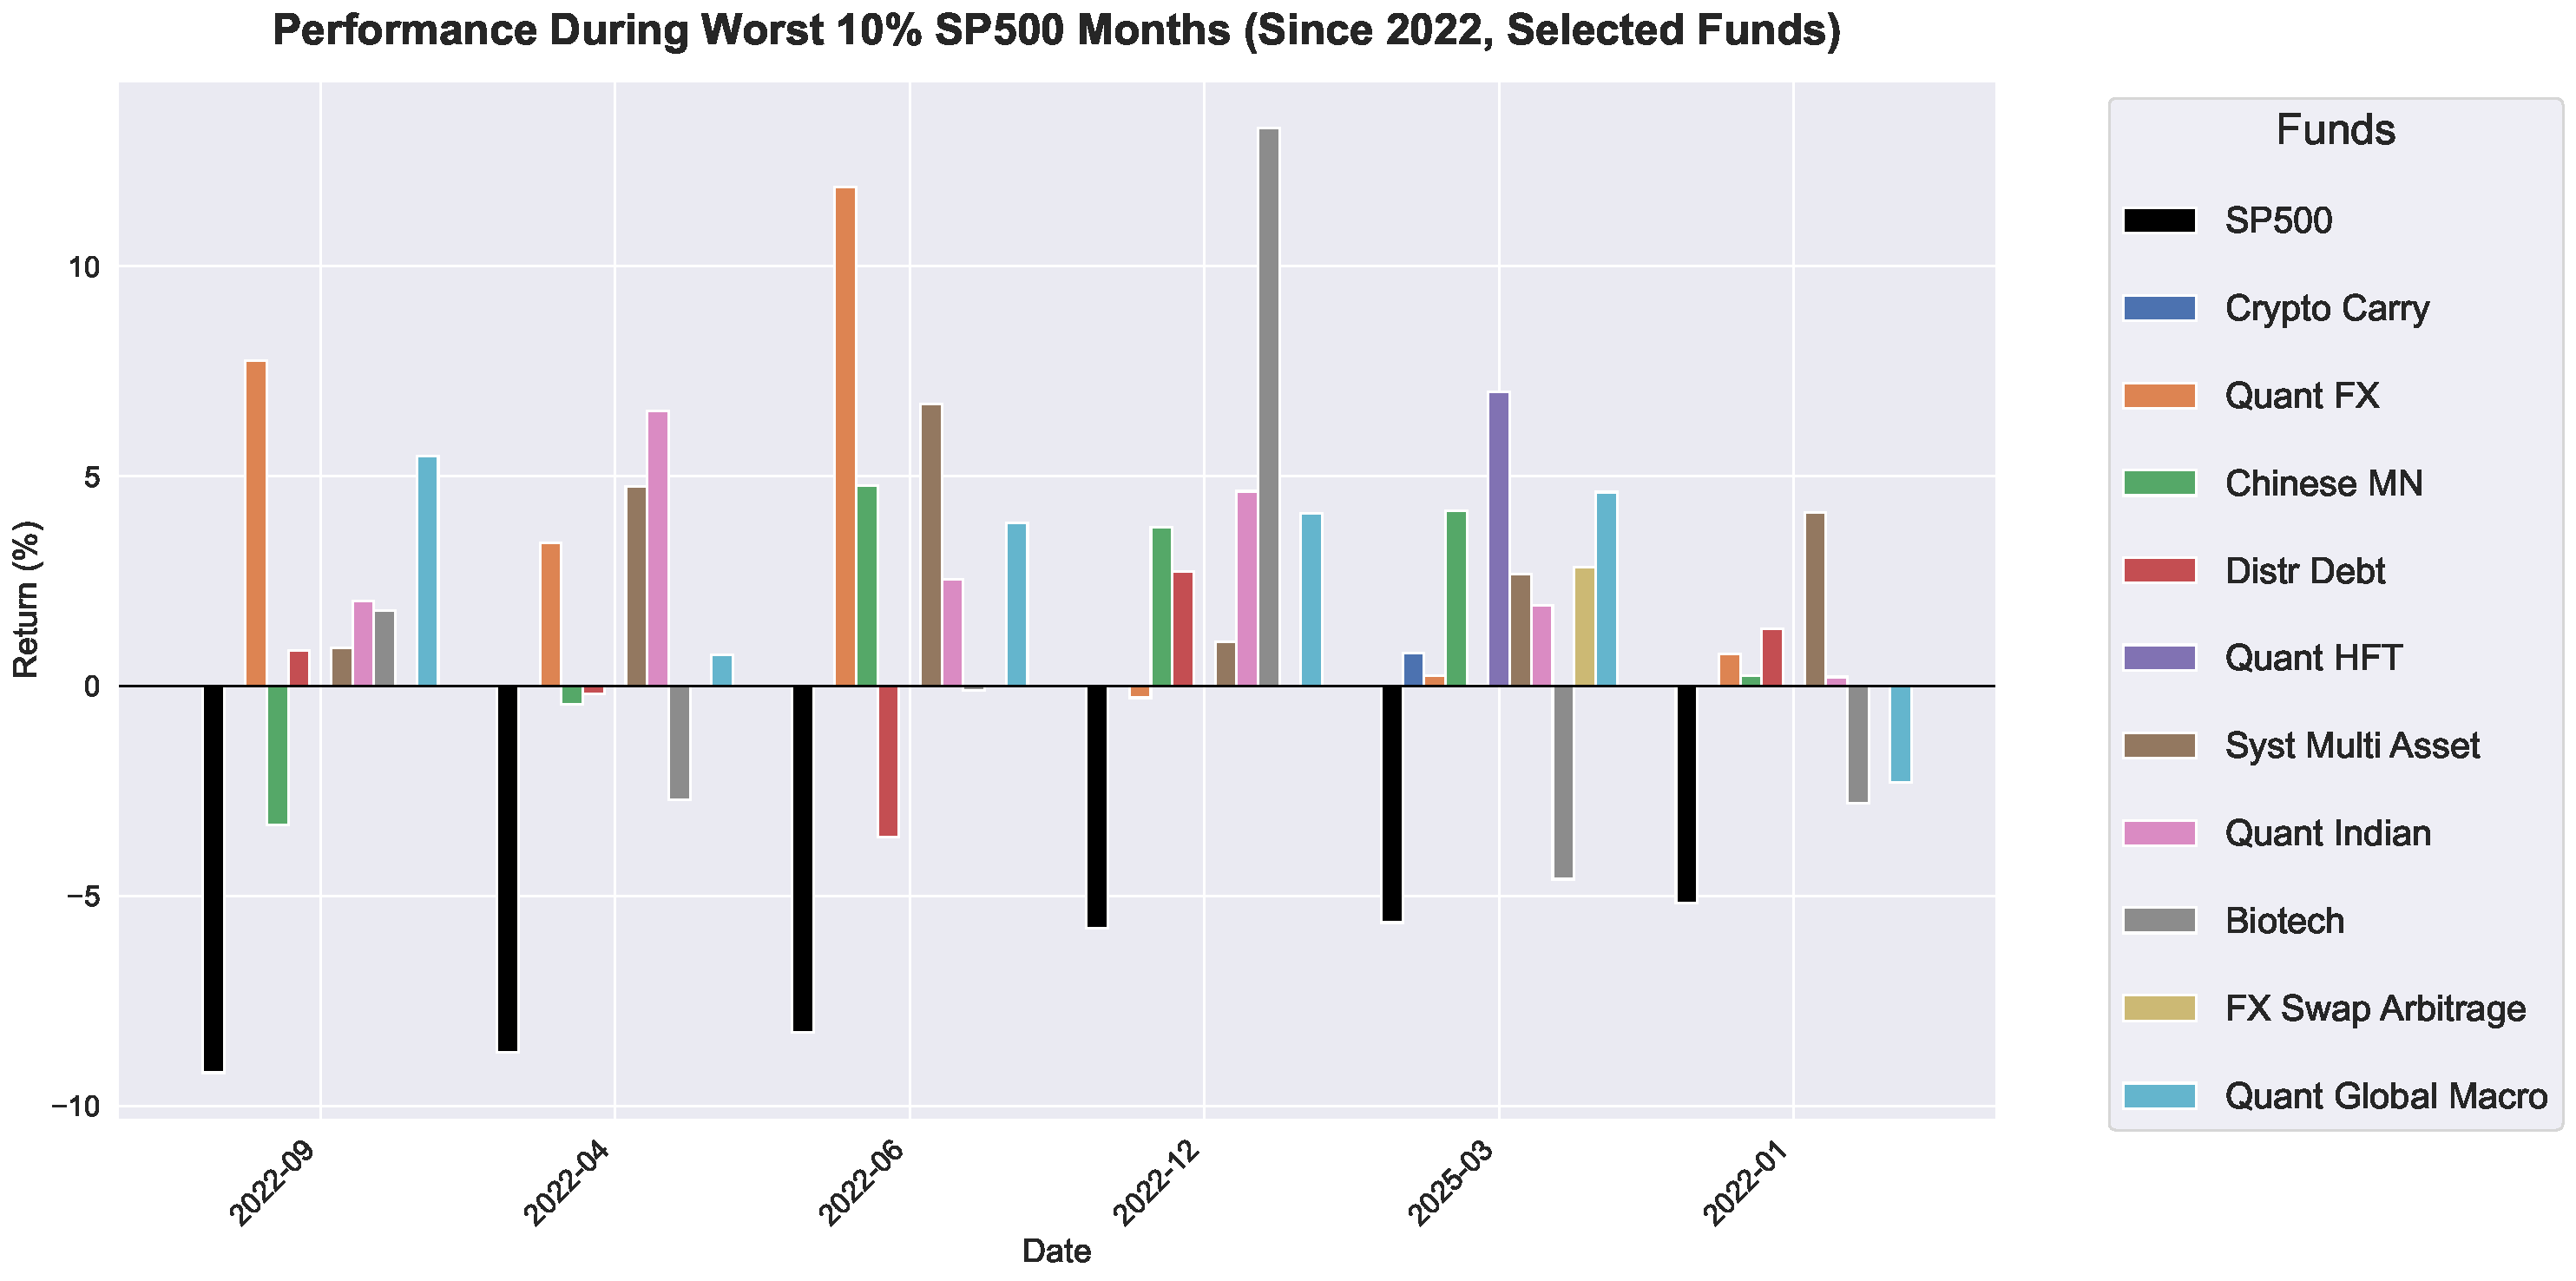
\includegraphics[width=0.95\textwidth, height=0.42\textheight, keepaspectratio]{worst_sp500_months.pdf}

    \vspace{0.5em}

    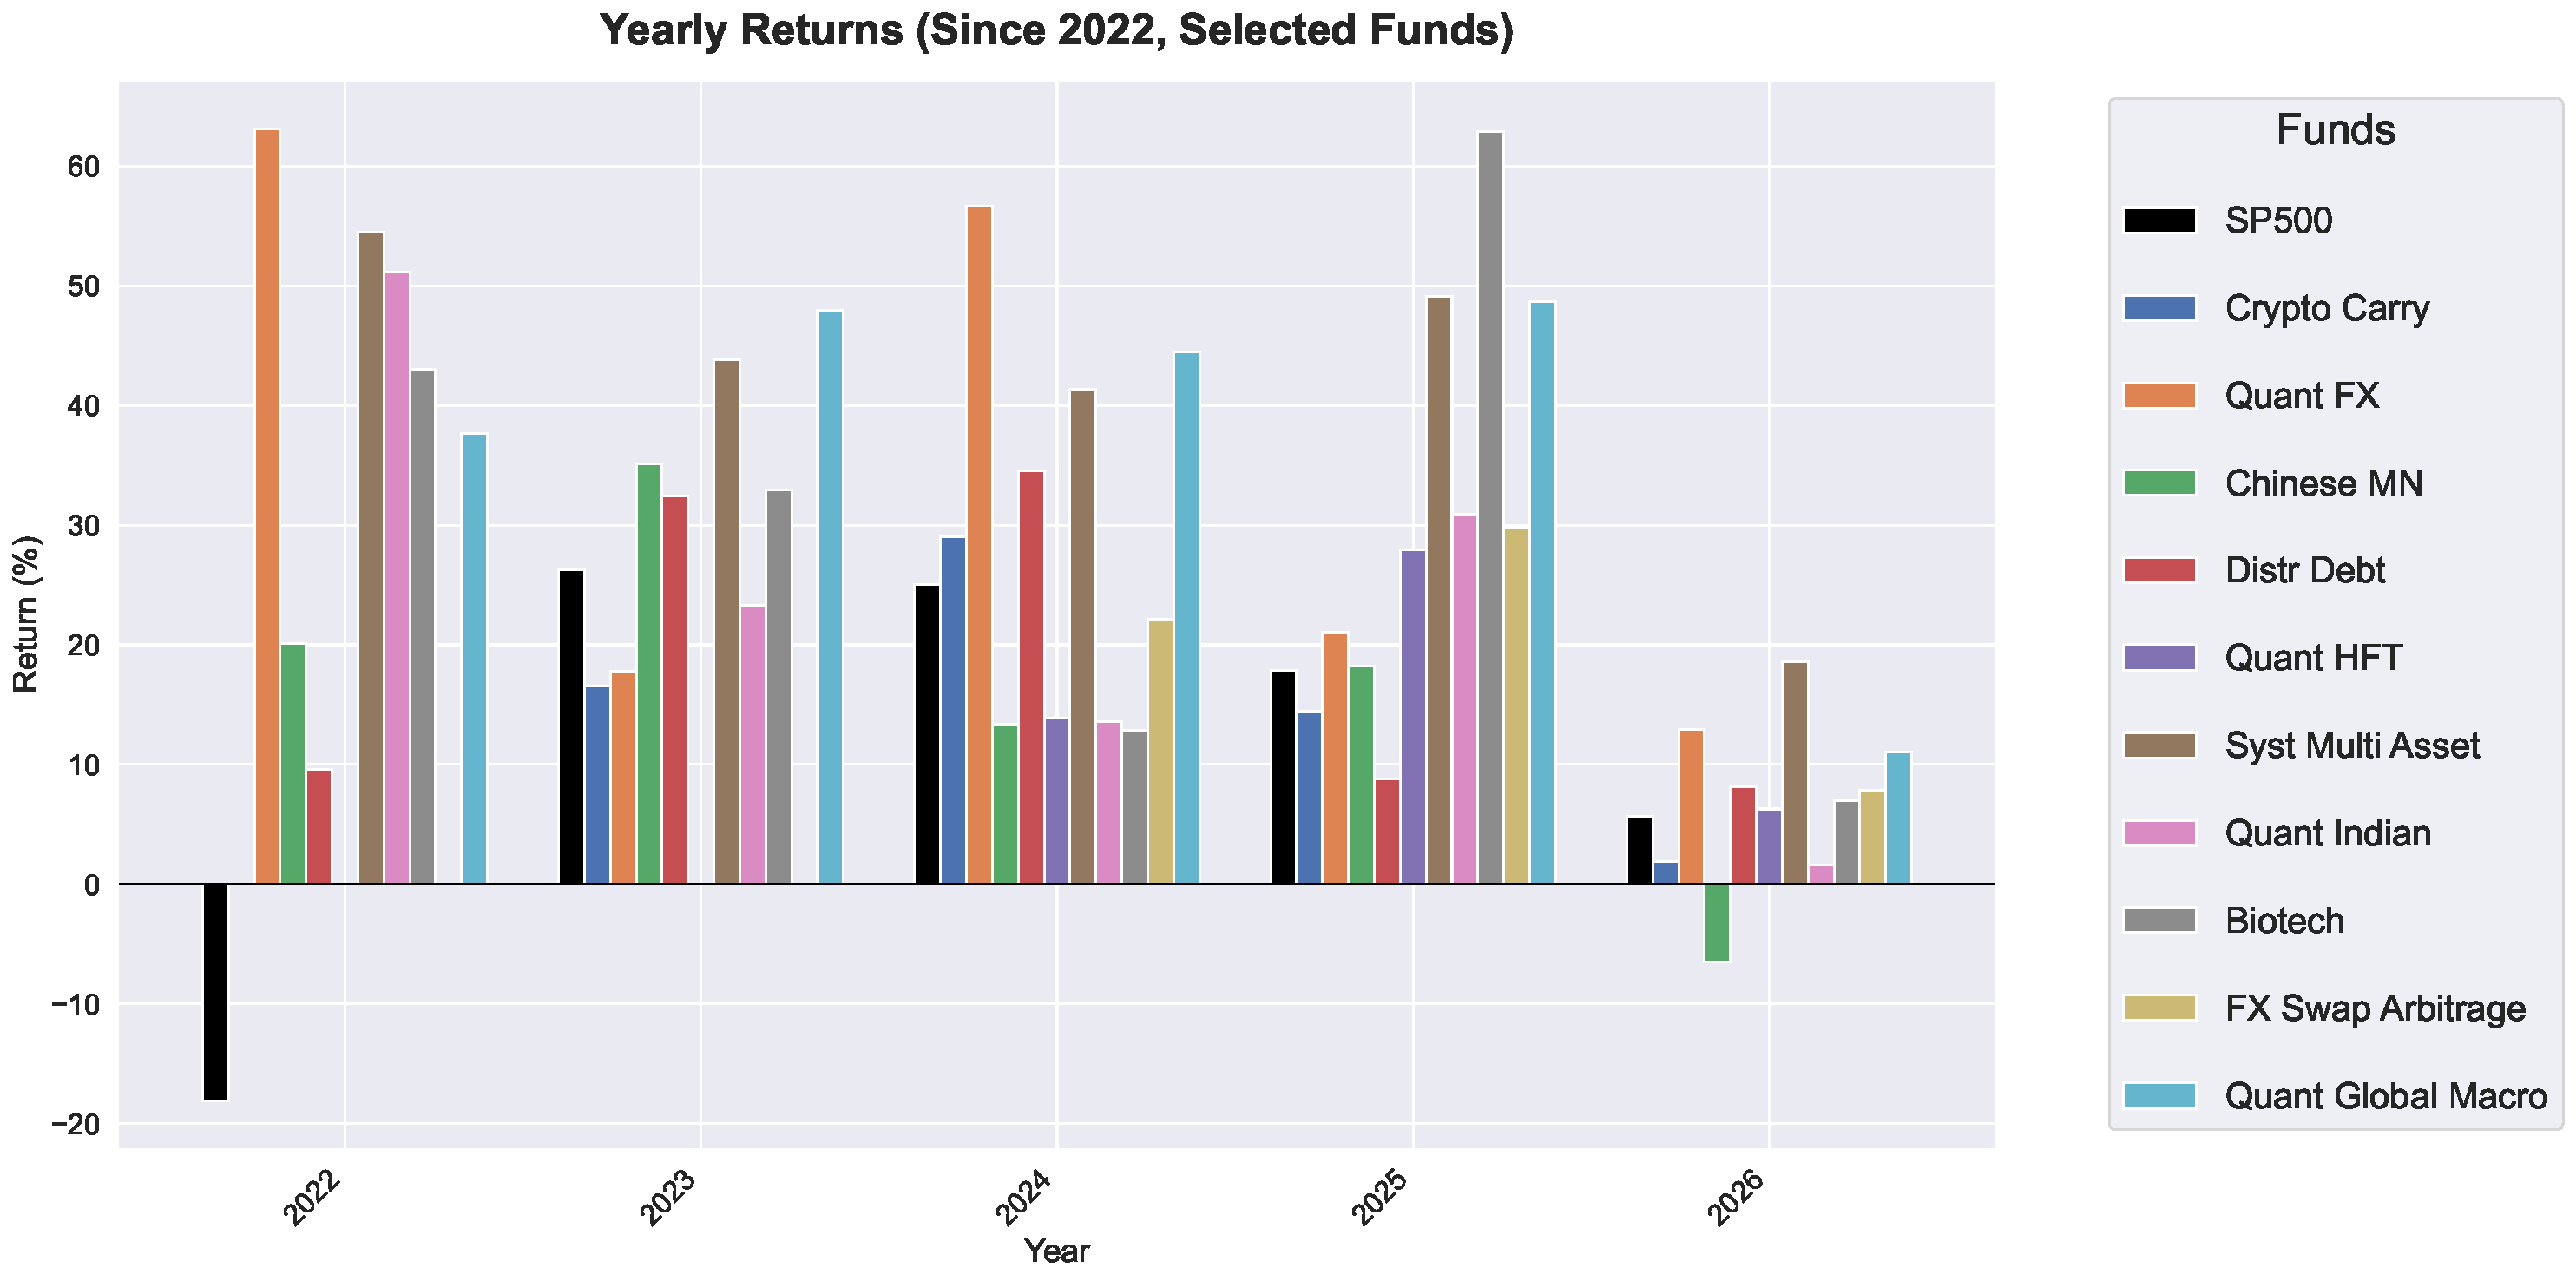
\includegraphics[width=0.95\textwidth, height=0.42\textheight, keepaspectratio]{yearly_returns_all_funds.pdf}
\end{center}

\clearpage
%%%%%%%%%%%%%%%%%%%%%%%%%%%%%%%%%%%%%%%%%%%%
%% LAST PAGE: Portfolio Backtest Methodologies
%%%%%%%%%%%%%%%%%%%%%%%%%%%%%%%%%%%%%%%%%%%%

\section*{Portfolio Growth Analysis}
Here we compare four portfolio weighting methodologies.

\begin{center}
    
\includegraphics[width=0.95\textwidth, height=0.4\textheight, keepaspectratio]{4_strategies_growth.pdf}

    \vspace{0.5em}

    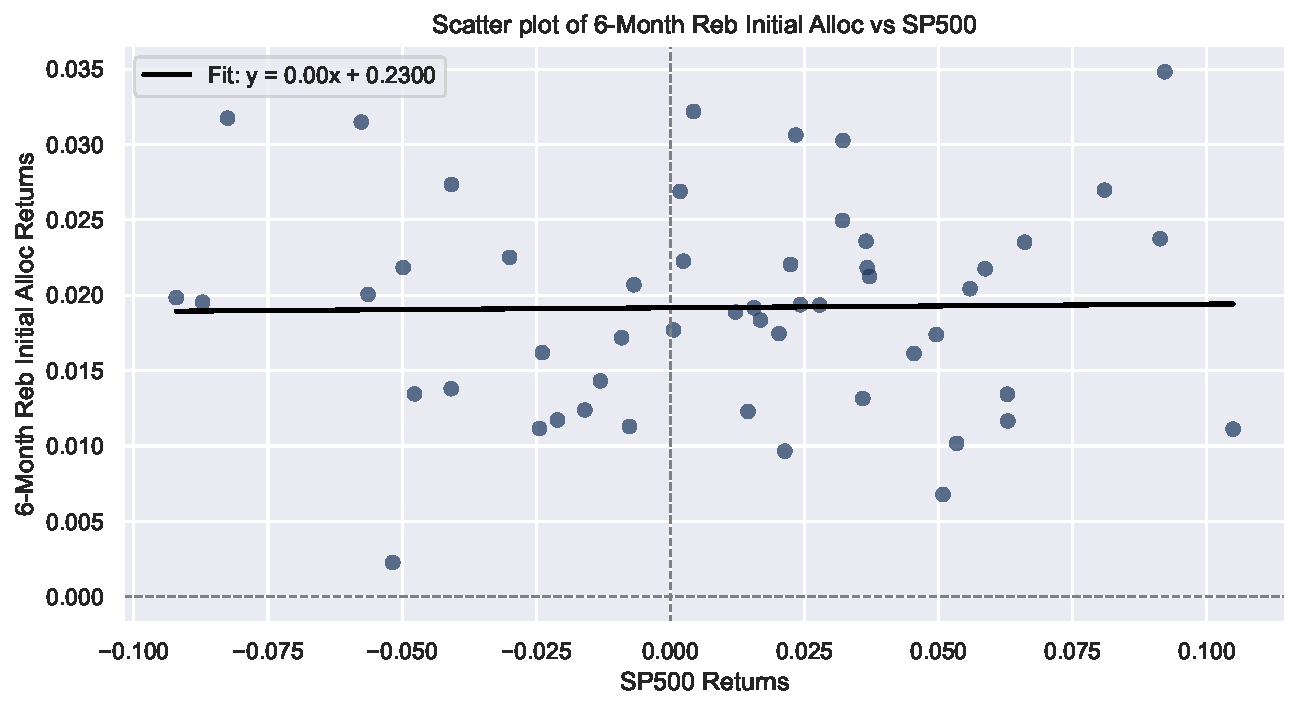
\includegraphics[width=0.95\textwidth, height=0.4\textheight, keepaspectratio]{scatter_6_month_reb_initial_alloc_vs_sp500.pdf}
\end{center}



\end{document}
